% ****** Start of file apssamp.tex ******
%
%   This file is part of the APS files in the REVTeX 4.1 distribution.
%   Version 4.1r of REVTeX, August 2010
%
%   Copyright (c) 2009, 2010 The American Physical Society.
%
%   See the REVTeX 4 README file for restrictions and more information.
%
% TeX'ing this file requires that you have AMS-LaTeX 2.0 installed
% as well as the rest of the prerequisites for REVTeX 4.1
%
% See the REVTeX 4 README file
% It also requires running BibTeX. The commands are as follows:
%
%  1)  latex apssamp.tex
%  2)  bibtex apssamp
%  3)  latex apssamp.tex
%  4)  latex apssamp.tex
%
\documentclass[%
 reprint,
%superscriptaddress,
%groupedaddress,
%unsortedaddress,
%runinaddress,
%frontmatterverbose, 
%preprint,
%showpacs,preprintnumbers,
%nofootinbib,
%nobibnotes,
%bibnotes,
 amsmath,amssymb,
 aps,
%pra,
%prb,
%rmp,
%prstab,
%prstper,
%floatfix,
]{revtex4-1}

\usepackage{graphicx}% Include figure files
\usepackage{dcolumn}% Align table columns on decimal point
\usepackage{bm}% bold math
%\usepackage{hyperref}% add hypertext capabilities
%\usepackage[mathlines]{lineno}% Enable numbering of text and display math
%\linenumbers\relax % Commence numbering lines

%\usepackage[showframe,%Uncomment any one of the following lines to test 
%%scale=0.7, marginratio={1:1, 2:3}, ignoreall,% default settings
%%text={7in,10in},centering,
%%margin=1.5in,
%%total={6.5in,8.75in}, top=1.2in, left=0.9in, includefoot,
%%height=10in,a5paper,hmargin={3cm,0.8in},
%]{geometry}

\graphicspath{{./images/}}
\newcommand{\x}[0]{\mathbf{x}}
\newcommand{\dx}[0]{\mathrm{d}\x}

\begin{document}

\preprint{APS/123-QED}

\title{Dropping Lowest and Highest Score in Debate Adjudication Processes}% Force line breaks with \\


\author{Ann Author}
 %\altaffiliation[Also at ]{Physics Department, XYZ University.}%Lines break automatically or can be forced with \\
 
\author{Bee Author}%
 %\email{Second.Author@institution.edu}
\affiliation{%Authors' institution and/or address
G\"ottingen Institute for Contemporary Debate Research
}%

\author{Cee Author}%
\email{corresponding.author@institution.edu}
\affiliation{%Authors' institution and/or address
	G\"ottingen Institute for Contemporary Debate Research
}%

\date{\today}% It is always \today, today,
             %  but any date may be explicitly specified

\begin{abstract}
Debating is a competetive sport where the winner is decided based upon points given from adjudicators. A common practice in sports with similar setup is to drop the highest and lowest scoring for each contestant. In this work, we take a statistical approach to analyze the effect of this measure on the example of the debating system \textit{Offene Parlamentarische Debatte}.
\end{abstract}

%\pacs{Valid PACS appear here}% PACS, the Physics and Astronomy
                             % Classification Scheme.
%\keywords{Suggested keywords}%Use showkeys class option if keyword
                              %display desired
\maketitle

%\tableofcontents

\section{\label{sec:level1}Introduction}

Debating is a highly competitive ... \textit{Offene Parlamentarische Debatte} (OPD) adjudicators ..., (cite Regelwerk)\\

Similar types of competitive sports exist where the sport does not include any direct quantitive measure (like e.g. goals in football), but rather the performance in a sport is decided through adjudicators and is based on criteria, where a full objective measure is not possible. A common procedure in a number of these sports is that for each player or participant, both the highest and the lowest rating are dropped. Examples are gymnastics \footnote{https://usagym.org/pages/events/pages/fig\_scoring.html}, ski jumping \footnote{https://www.pyeongchang2018.com/en/sports/ski-jumping} and diving competitions \footnote{http://www.nbcolympics.com/news/diving-101-scoring}. \\

In the preliminary rounds often a high difference in experience is present, which is accounted for by the chief adjudicators and chairs ...  We therefore focus on the judging of finals (and potentially quarter and semi finals, if existant), where the so called \textit{break} assures a certain standarization ... In addition, for simplicity, we solely focus on a single integer, the total speaker points, as well as the points of a team, that is the sum of three speaker points. We, however, believe the results will without loss of generality be usable for team points or single speaker categories. 

We make the following assumptions:
\begin{enumerate}
	\item Every adjudicator awards all points to the best of his / her knowledge and abilities. This means in no case does any adjudicator award points despite the knowledge that they do not match the speaker's or the team's performance. 
	\item No communication between adjudicators. If the results, and especially the adjudicators who have given the highest and lowest points, change during the adjudication discussion, this may have implications. For now, this study will focus on speakers whose result are not discussed in the panel.  
	\item The ``true'' strength of a speaker is defined by the average number points that a speaker would get from a high or infinite number of adjudicators with the experience to break into a final. 
	\item The points awarded by an adjudicator spread in a Gaussian fashion for a single speaker. This means, that if the same adjudicator would listen to the identical speech again (without remembering) he / she would probably not give identical points, but rather a number drawn from a probablility distribution spread around a mean that would be reached if the adjudicator was (conceptually) allowed to listen to the same speech an infinite number of times. 
	\item This aformentioned mean again is spreaded for different adjudicators. It is openly recognized that different adjudicators award systematically higher  or lower points than others. 
\end{enumerate}

We assume the distribution of point 4. and 5. as Gaussian. This is justified through the Central Limit Theorem, that states that for a high number of parameters ..., the probability distribution always approaches a Gaussian. In OPD, five categories go into the total speaker points, while a large number of criteria, that is differently evaluated and weighted by each adjudicator, contributes to each category. 

\section{Analytical Considerations}

\subsection{Single Adjudicator}

A single speaker has a true strength of $\mu_{true}$.The adjudicator $n$ has a point level of $\mu_n$. It is drawn from a Gaussian distribution with mean $\mu_{true}$, and standard deviation $\sigma_s$, i.e. the probability density function (PDF) is
\begin{equation}
p(\mu_n | \mu_{true}) = \frac{1}{\sqrt{2\pi} \sigma_s} \exp\left(-\frac{(\mu_n - \mu_{true})^2}{2\sigma_s^2}\right)
\label{eq:01_ideal_panel}
\end{equation}
Equation~\ref{eq:01_ideal} therefore gives the distribution that would be obtained for an infinite number of adjudicators is therefore centred around the true value. The speaker points awarded for the speaker by adjudicator $n$ denoted by $x_n$ is again drawn from a Gaussian distribution with mean $\mu_n$ and $\sigma_n$:
\begin{equation}
p(x_n | \mu_n) = \frac{1}{\sqrt{2\pi} \sigma_n} \exp\left(-\frac{(x_n - \mu_n)^2}{2\sigma_n^2}\right)
\label{eq:02_single_adjudication}
\end{equation}
Equation~\ref{eq:02_single_adjudication} reflects the fact that an adjudicator has a some uncertainty, i.e. would possibly award the same speech different points each time he / she saw and forgot it agian. Now, the probability density function for such a speaker is the convolution of equation~\ref{eq:01_ideal_panel} and equation~\ref{eq:02_single_adjudication} and integrating out the probability to obtain a certain adjudicator. 
\begin{align}
p(x_n|\mu_{true}) =& \int_0^{100} d\mu_n\: p(x_n|\mu_n)\: p(\mu_n|\mu_{true})\\
\end{align}

%\begin{align}
%p(x_n|\mu_{true}) =& \frac{1}{2\pi\sigma_s\sigma_n}\int_0^{100} d\mu_n\\
%&\cdot \exp\left(...\right)
%\label{eq:03_combined}
%\end{align}
The combination of the terms again leads to the form of a Gaussian integral. The integration is conducted for bounds of $\pm \infty$. We assume the probability density around the real bounds of 0 and 100 sufficiently small, such that the contribution of the integral beyond these points is negligible. The solution is calculated as:

\begin{align}
p(x_n|\mu_{true}) =\frac{1}{2\pi\sigma_s\sigma_n} \sqrt{\frac{\pi}{a}}\exp\left(\frac{b^2}{4a}+c\right)\\
\end{align}
with
\begin{align}
a(\sigma_n, \sigma_s) &= \frac{1}{2}\left(\frac{1}{\sigma_s^2} + \frac{1}{\sigma_n^2}\right)\\
b(x_n, \sigma_n, \sigma_s, \mu_{true}) &= \frac{x_n}{\sigma_s^2} + \frac{\mu_{true}}{\sigma_n^2}\\
c(x_n, \sigma_n, \sigma_s, \mu_{true}) &= -\frac{1}{2}\left(\frac{x_n^2}{\sigma_s^2} + \frac{\mu_{true}^2}{\sigma_n^2}\right)
\end{align}

The probability function over $x_n$ can be evaluated, given the parameters $\sigma_s$, $\sigma_n$ and $\mu_{true}$. We show a plot for an example range of parameters in figure xy.\\

\subsection{Multiple Adjudicators}




\subsubsection{Without Point Dropping}
For a number of adjudicators $N$, the resulting score $\bar{x}$ calculated through a simple average, i.e.
\begin{align}
\bar{x} = \frac{1}{N}\sum_{n=1}^{N} x_n
\end{align}
Therefore, assuming the points are uncorrelated (no communication between adjudicators) the PDF for the total score can be calculated as
\begin{align}
p(\bar{x}|\mu_{true}) = \frac{1}{Z}\prod_{n=1}^{N}p(x_n|\sigma_n, \sigma_s, \mu_{true})
\end{align}
where $Z$ is the normalization constant, i.e.
\begin{align}
Z = \int_\Gamma \prod_{n=1}^{N}p(x_n|\sigma_n, \sigma_s, \mu_{true})
\end{align}
where the integration is conducted over whole $\Gamma$, which denotes the adjudication space of dimension $N$. Again, this can easily be evaluated for a given set of parameters and examples are shown in figure xyz. \\

Now, we calculate the accuracy of the method through 
\begin{align}
<(\bar{x} - \mu_{true})>
\end{align}

\subsubsection{With Point Dropping}

Now, we introduce a function $f(x_n)$ with 
\begin{align}
f(x_n) &= 0 \;\; \text{if} \;\; x_n \;\; \text{smallest or highest element}\\
&= 1 \;\; \text{else} 
\end{align}

Now, analogous to before:
\begin{align}
\bar{x} = \frac{1}{N-2}\sum_{n=1}^{N} f(x_n)
\end{align}
For the adjudication space, this means a projection of $\Gamma_N \rightarrow \Gamma_{N-2}$, i.e. from the $N$ dimensional space to the $N-2$ dimensional space. 


\section{Numerical Validation}

We here simulate a high number of finals (excluding independent speakers). It is the goal to compare the accuracy of the two aforementioned methods.
\subsection{Single Speaker}
 The true value is assigned to 50. Procedure:
\begin{itemize}
	\item Draw five values $\mu_i$ discrete values from a Gaussian distribution with mean 50 and standard deviation $\sigma_s$. These are the means of the adjudicators.
	\item For each adjudicator, draw a value $x_n$ from a Gaussian distribution with mean $\mu_n$ and standard deviation $\sigma_n$. 
	\item Combine the points to $\bar{x}$ and calculate the squared deviation to the true value $\mu_{true}$.
	\item Simulate a high number of finals and take the mean (and std) of the squared deviations. We thus obtain $<(\bar{x} - \mu_{true})^2>$
	\item One time $\sigma_s$ is varied, another time, $\sigma_n$ is varied.
\end{itemize}

\begin{figure}[hbt!]
	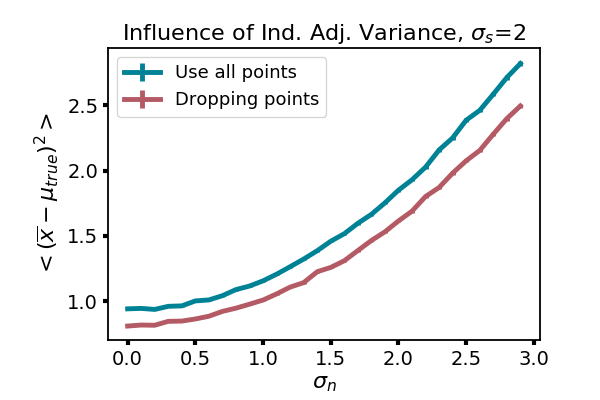
\includegraphics[width=\linewidth]{single_speaker_sigma_s_2_var_sigma_n}
	\caption{Varying the standard deviation of the individual adjudicator $\sigma_n$ (assumed equal for each adjudicator). The average point level of each adjudicator is drawn from a distribution centered on $\mu_{true}=50$ and with $\sigma_s=2$. Dropping the highest and lowest points leads to a better result in all cases. 50,000 final simulations were conducted.}
	\label{fig:single_speaker_vary_sigma_n}
\end{figure}

\begin{figure}[hbt!]
	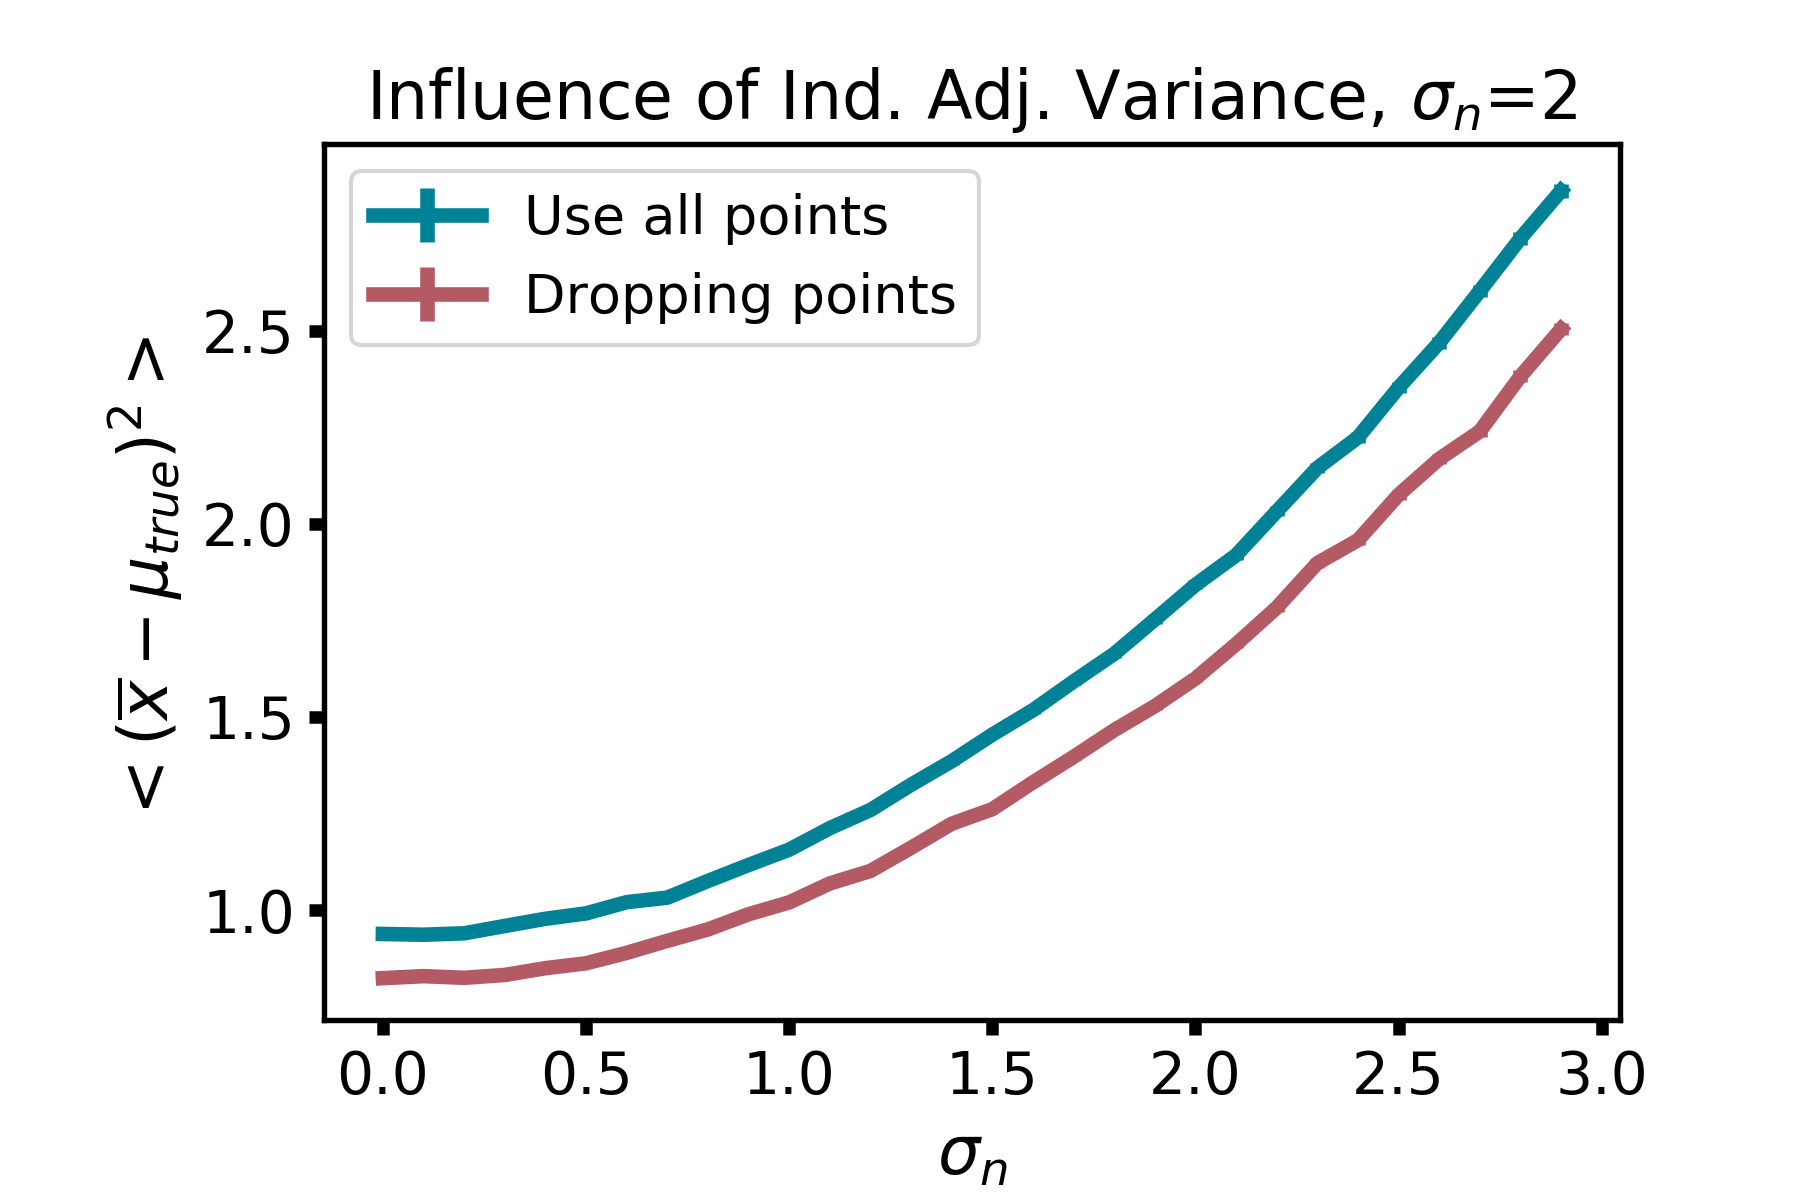
\includegraphics[width=\linewidth]{single_speaker_var_sigma_s_sigma_n_2}
	\caption{Varying the standard deviation of the different point level of the adjudicators $\sigma_s$. The standard deviation of each individual adjudicator is kept constant at $\sigma_n = 2$. Dropping the highest and lowest points leads to a better result in all cases. 50,000 final simulations were conducted.}
	\label{fig:single_speaker_vary_sigma_s}
\end{figure}
%Convoluted Gaussian

\subsection{Team Win}

Procedure:



\section{Conclusion}

\begin{acknowledgments}
%We wish to acknowledge the support of the author community in using
%REV\TeX{}, offering suggestions and encouragement, testing new versions,
%\dots.
\end{acknowledgments}

\appendix

\section{Appendixes}



\bibliography{apssamp}% Produces the bibliography via BibTeX.

\end{document}
%
% ****** End of file apssamp.tex ******
